\documentclass[10pt,a4paper]{article}
\usepackage[utf8]{inputenc}
\usepackage[english]{babel}
%\usepackage{minted}
\usepackage{listings}
\usepackage{xcolor}
\usepackage{graphicx}

%For syntax highlighting
\definecolor{codegreen}{rgb}{0,0.6,0}
\definecolor{codegray}{rgb}{0.5,0.5,0.5}
\definecolor{codepurple}{rgb}{0.58,0,0.82}
\definecolor{backcolour}{rgb}{1,1,1}

%%Sets different parameters
\lstdefinestyle{mystyle}{
	backgroundcolor=\color{backcolour},   
    commentstyle=\color{codegreen},
    keywordstyle=\color{magenta},
    numberstyle=\tiny\color{codegray},
    stringstyle=\color{codepurple},
    basicstyle=\ttfamily\footnotesize,
    breakatwhitespace=false,         
    breaklines=true,                 
    captionpos=b,                    
    keepspaces=true,                 
    numbers=left,                    
    numbersep=5pt,                  
    showspaces=false,                
    showstringspaces=false,
    showtabs=false,                  
    tabsize=4
}
\lstset{style=mystyle}

\title{\bf Matrix Operations}
\author{\vspace{-10ex}}
\date{\vspace{-10ex}}
\begin{document}
\maketitle

\begin{minipage}{0.45\textwidth}
        \begin{tabular}{l l}
            \textbf{Expt No:}&5\\
            \textbf{Date :}&09/10/2020
        \end{tabular}
\end{minipage}%
\begin{minipage}{0.45\textwidth}
        \begin{tabular}{l l}
             \textbf{Name:}& Shivanirudh S G  \\
             \textbf{Reg No:} & 185001146 
        \end{tabular}
\end{minipage}
\vspace{1cm}
\hrule

\begin{flushleft}
\subsection*{\textbf{Aim:}} 
To perform matrix operations in 8086.

\vspace{1cm}
\hrule
\subsection*{\textbf{\underline{Matrix Addition}}}

\subsubsection*{\textbf{Algorithm:}}
\begin{itemize}
    \item Move the data segment to the AX register and then move it to the DS register.
    \item Move offsets of mat1, mat2 and mat3 into SI, DI, BX registers respectively.
    \item Move value of count to CX register
    \item Move values of r1, r2, c1, c2 into AL, AH, DL, DH registers respectively. 
    \item Compare AL, AH by CMP AL, AH and jump to exit if unequal.
    \item Compare BL, BH by CMP BL, BH and jump to exit if unequal.
    \item Move value at [SI] to AL register.
    \item Add AL with value at [DI].
    \item Move value at AL to [BX].
    \item Increment SI, DI and BX, decrease CX, repeat till CX = 0.
\end{itemize}

\newpage
\subsubsection*{\textbf{Program:}}

\begin{table}[htb]
\centering
\resizebox{\columnwidth}{!}{
\begin{tabular}{|l|l|} 
\hline
\textbf{Program}                                                 & \textbf{Comments}                             \\ 
\hline
\hline
assume cs:code, ds:data                                          & Declare code and data segments                \\
\hline
data segment                                                     & Start of data segment                         \\
\hline
r1 db 02H                                                        & Define byte r1 with value 02H                 \\
\hline 
r2 db 02H                                                        & Define byte r2 with value 02H                 \\
\hline
c1 db 03H                                                        & Define byte c1 with value 03H                 \\
\hline
c2 db 03H                                                        & Define byte c2 with value 03H                 \\
\hline
count dw 0006H                                                   & Define word count with value 0006H            \\
\hline
mat1 db 22H, 33H, 44H, 55H, 66H, 77H                             & Define matrix of values mat1                  \\
\hline
mat2 db 33H, 44H, 55H, 66H, 77H, 88H                             & Define matrix of values mat2                  \\
\hline 
mat3 db ?                                                        & Define result matrix of values mat3           \\
\hline
data ends                                                        & End of data segment                           \\
\hline
code segment                                                     & Start of code segment                         \\
\hline
start:~mov ax, data                                              & Move data to AX register                      \\
\hline
mov ds, ax                                                       & Move contents of AX register to DS register   \\
\hline
mov dl, 0AH                                                      & Move hex value 0A to DL register              \\
\hline
mov si, offset mat1                                              & Move offset of mat1 to SI register            \\
\hline
mov di, offset mat2                                              & Move offset of mat2 to DI register            \\
\hline
mov bx, offset mat3                                              & Move offset of mat3 to BX register            \\
\hline
mov cx, count                                                    & Move value of count to CX register            \\
\hline
mov al, r1                                                       & Move value of r1 to AL register               \\
\hline
mov ah, r2                                                       & Move value of r2 to AH register               \\
\hline
mov dl, c1                                                       & Move value of c1 to DL register               \\
\hline
mov dh, c2                                                       & Move value of c2 to DH register               \\ 
\hline
cmp al, ah                                                       & Compare values of AL and AH registers         \\
\hline
jne exit                                                         & Jump to exit if ZF = 0                        \\
\hline
cmp dl, dh                                                       & Compare values of DL, DH registers            \\
\hline
jne exit                                                         & Jump to exit if ZF = 0                        \\
\hline
here:~mov al, [si]                                               & Move contents at SI to AL register            \\
\hline            
add al, [di]                                                     & AL = AL + [DI]                                \\
\hline
mov [bx], al                                                     & Move contents of AL register to BX register   \\
\hline
inc si                                                           & Increment value in SI register                \\
\hline 
inc di                                                           & Increment value in DI register                \\
\hline
inc bx                                                           & Increment value in BX register                \\         
\hline
dec cx                                                           & Decrement value of CX register                \\
\hline
jnz here                                                         & Jump to here if ZF = 0                        \\
\hline
exit:~mov ah, 4ch                                                & To request interrupt                          \\
\hline
int 21h                                                          & Request interrupt routine                     \\ 
\hline
code ends                                                        & End of code segment                           \\
\hline
end start                                                        &                                               \\
\hline
\end{tabular}
}
\end{table}

\newpage
\subsection*{\textbf{Unassembled code:}}
\begin{figure}[h]
    \centering
    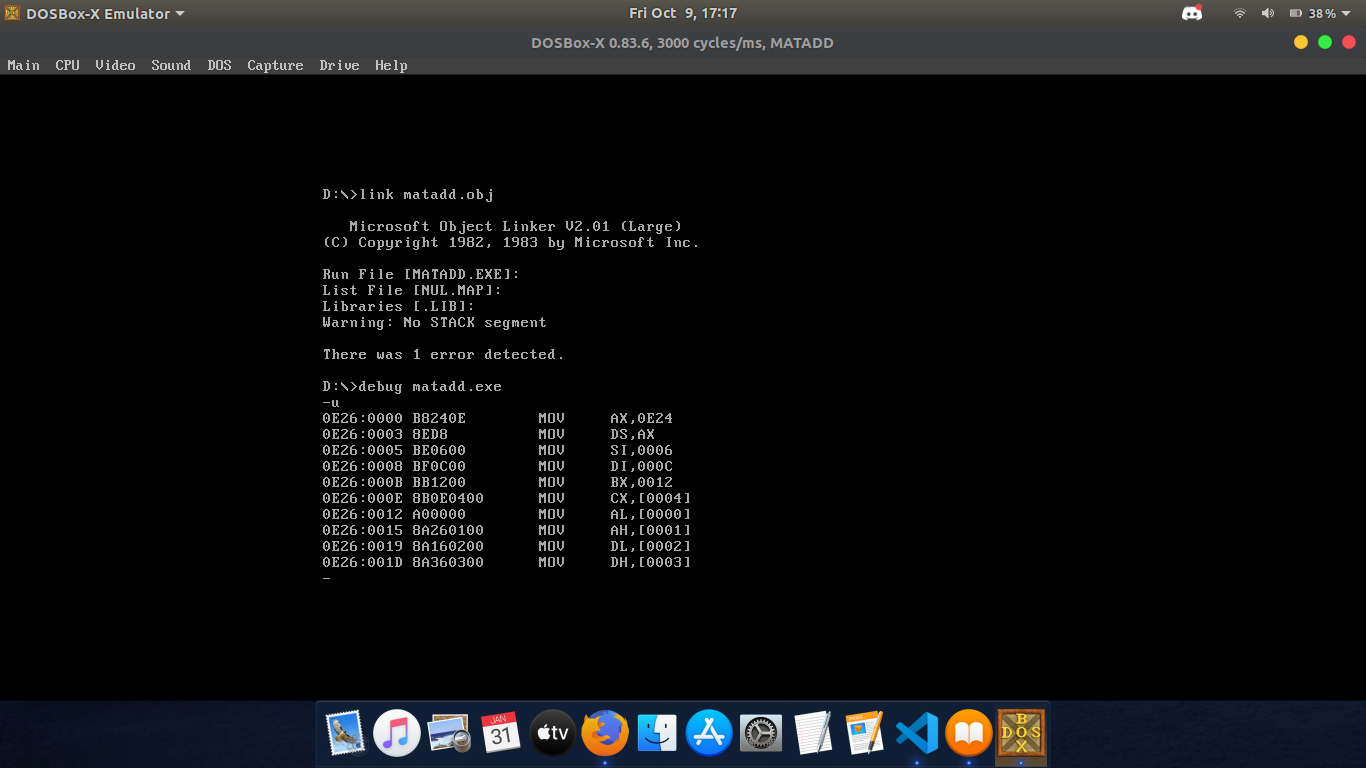
\includegraphics[trim = 100mm 60mm 200mm 120mm, clip, width = \textwidth]{Pics/MAUS.png}
\end{figure}
\subsubsection*{\textbf{Input and Output:}}
\begin{figure}[h]
    \centering
    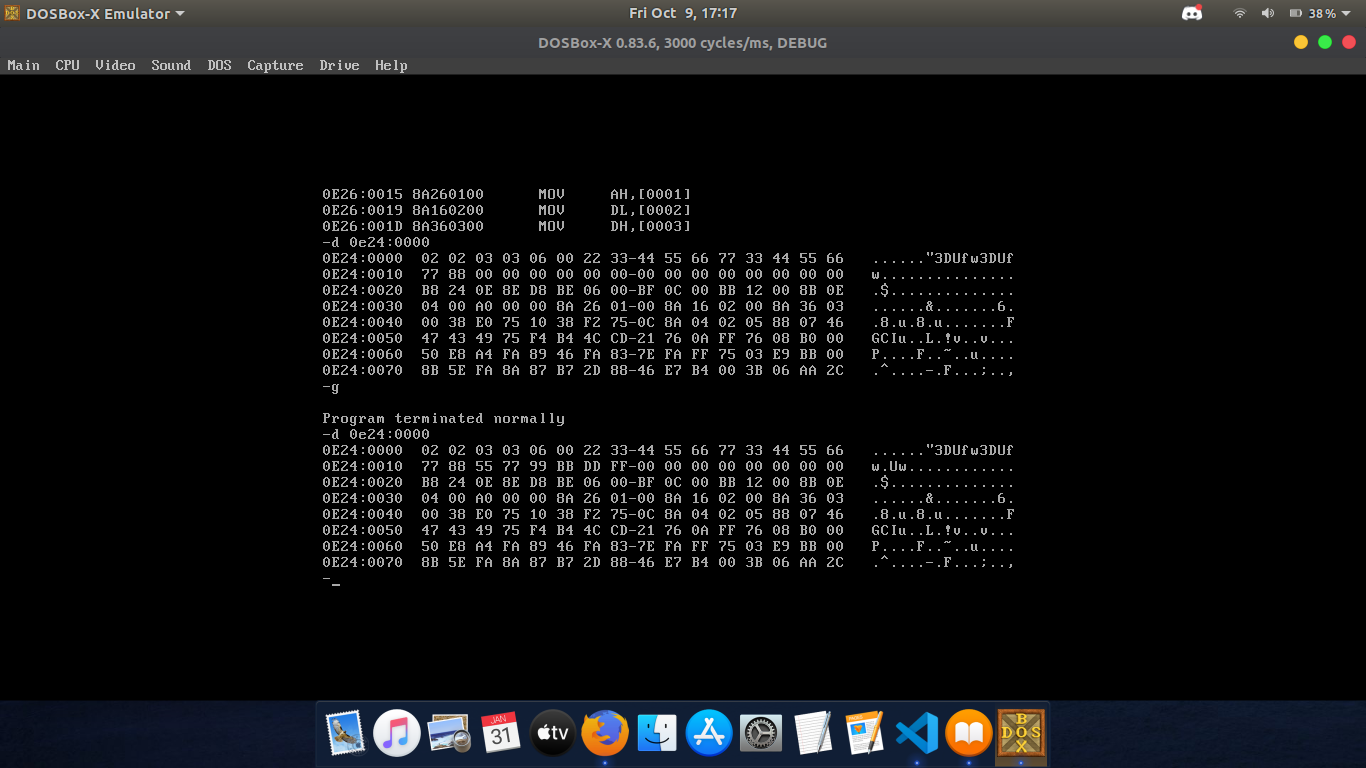
\includegraphics[trim = 100mm 60mm 100mm 80mm, clip, width = \textwidth]{Pics/MAIO.png}
    \caption{ \textbf{Input:} \emph{mat1:} 22H, 33H, 44H, 55H, 66H, 77H; \emph{mat2:} 33H, 44H, 55H, 66H, 77H, 88H ; \newline \hspace{1cm}
              \textbf{Output:} \emph{mat3:} 55H, 77H, 99H, BBH, DDH, FFH}
\end{figure}
%-------------------------------------------------------------------------------------------------------------------------------------------
\hrule
\newpage
\subsection*{\textbf{\underline{Matrix Subtraction}}}

\subsubsection*{\textbf{Algorithm:}}
\begin{itemize}
    \item Move the data segment to the AX register and then move it to the DS register.
    \item Move offsets of mat1, mat2 and mat3 into SI, DI, BX registers respectively.
    \item Move value of count to CX register
    \item Move values of r1, r2, c1, c2 into AL, AH, DL, DH registers respectively. 
    \item Compare AL, AH by CMP AL, AH and jump to exit if unequal.
    \item Compare BL, BH by CMP BL, BH and jump to exit if unequal.
    \item Move value at [DI] to AL register.
    \item Subtract AL with value at [SI].
    \item Move value at AL to [BX].
    \item Increment SI, DI and BX, decrease CX, repeat till CX = 0.
\end{itemize}

\newpage
\subsubsection*{\textbf{Program:}}

\begin{table}[htb]
\centering
\resizebox{\columnwidth}{!}{
\begin{tabular}{|l|l|} 
\hline
\textbf{Program}                                                 & \textbf{Comments}                             \\ 
\hline
\hline
assume cs:code, ds:data                                          & Declare code and data segments                \\
\hline
data segment                                                     & Start of data segment                         \\
\hline
r1 db 02H                                                        & Define byte r1 with value 02H                 \\
\hline 
r2 db 02H                                                        & Define byte r2 with value 02H                 \\
\hline
c1 db 03H                                                        & Define byte c1 with value 03H                 \\
\hline
c2 db 03H                                                        & Define byte c2 with value 03H                 \\
\hline
count dw 0006H                                                   & Define word count with value 0006H            \\
\hline
mat1 db 22H, 33H, 44H, 55H, 66H, 77H                             & Define matrix of values mat1                  \\
\hline
mat2 db 33H, 44H, 55H, 66H, 77H, 88H                             & Define matrix of values mat2                  \\
\hline 
mat3 db ?                                                        & Define result matrix of values mat3           \\
\hline
data ends                                                        & End of data segment                           \\
\hline
code segment                                                     & Start of code segment                         \\
\hline
start:~mov ax, data                                              & Move data to AX register                      \\
\hline
mov ds, ax                                                       & Move contents of AX register to DS register   \\
\hline
mov dl, 0AH                                                      & Move hex value 0A to DL register              \\
\hline
mov si, offset mat1                                              & Move offset of mat1 to SI register            \\
\hline
mov di, offset mat2                                              & Move offset of mat2 to DI register            \\
\hline
mov bx, offset mat3                                              & Move offset of mat3 to BX register            \\
\hline
mov cx, count                                                    & Move value of count to CX register            \\
\hline
mov al, r1                                                       & Move value of r1 to AL register               \\
\hline
mov ah, r2                                                       & Move value of r2 to AH register               \\
\hline
mov dl, c1                                                       & Move value of c1 to DL register               \\
\hline
mov dh, c2                                                       & Move value of c2 to DH register               \\ 
\hline
cmp al, ah                                                       & Compare values of AL and AH registers         \\
\hline
jne exit                                                         & Jump to exit if ZF = 0                        \\
\hline
cmp dl, dh                                                       & Compare values of DL, DH registers            \\
\hline
jne exit                                                         & Jump to exit if ZF = 0                        \\
\hline
here:~mov al, [di]                                               & Move contents at DI to AL register            \\
\hline            
add al, [si]                                                     & AL = AL - [SI]                                \\
\hline
mov [bx], al                                                     & Move contents of AL register to BX register   \\
\hline
inc si                                                           & Increment value in SI register                \\
\hline 
inc di                                                           & Increment value in DI register                \\
\hline
inc bx                                                           & Increment value in BX register                \\         
\hline
dec cx                                                           & Decrement value of CX register                \\
\hline
jnz here                                                         & Jump to here if ZF = 0                        \\
\hline
exit:~mov ah, 4ch                                                & To request interrupt                          \\
\hline
int 21h                                                          & Request interrupt routine                     \\ 
\hline
code ends                                                        & End of code segment                           \\
\hline
end start                                                        &                                               \\
\hline
\end{tabular}
}
\end{table}

\newpage
\subsection*{\textbf{Unassembled code:}}
\begin{figure}[h]
    \centering
    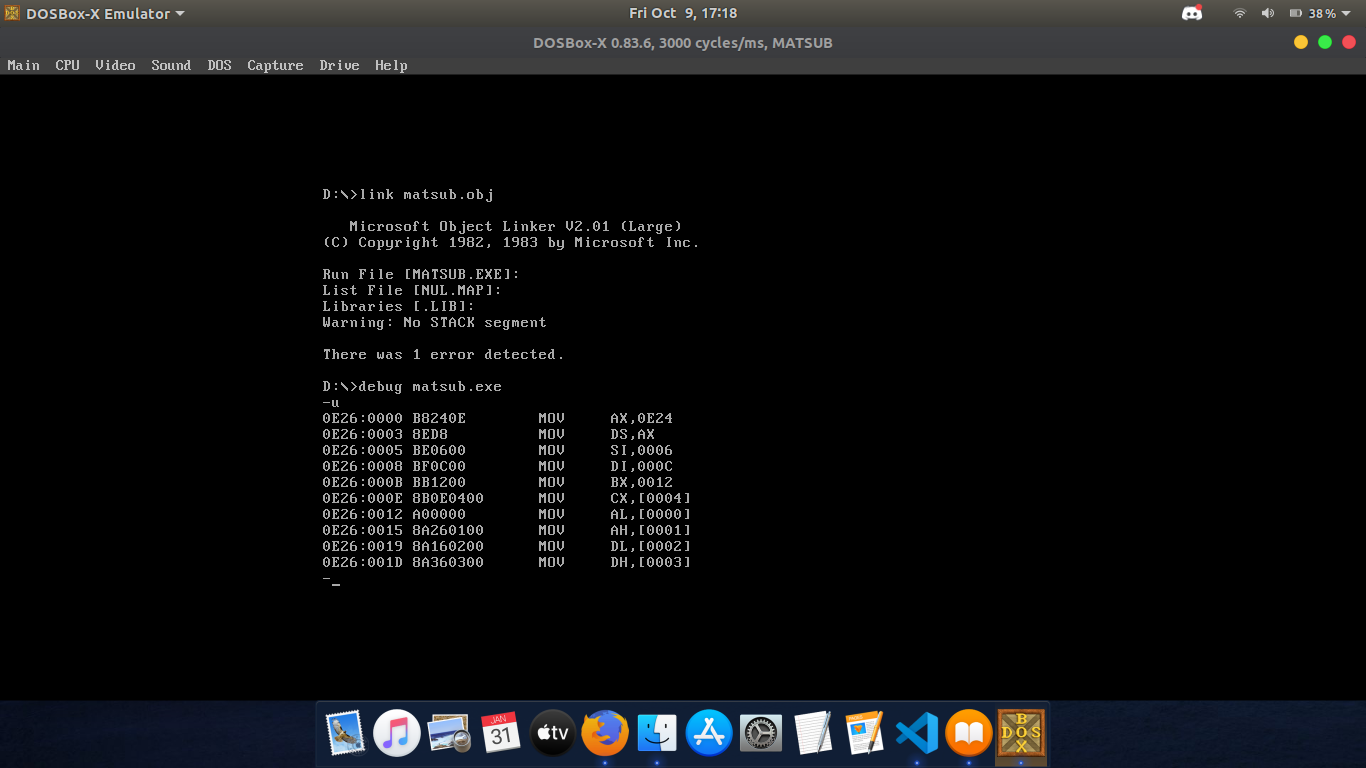
\includegraphics[trim = 100mm 60mm 200mm 120mm, clip, width = \textwidth]{Pics/MSUS.png}
\end{figure}
\subsubsection*{\textbf{Input and Output:}}
\begin{figure}[h]
    \centering
    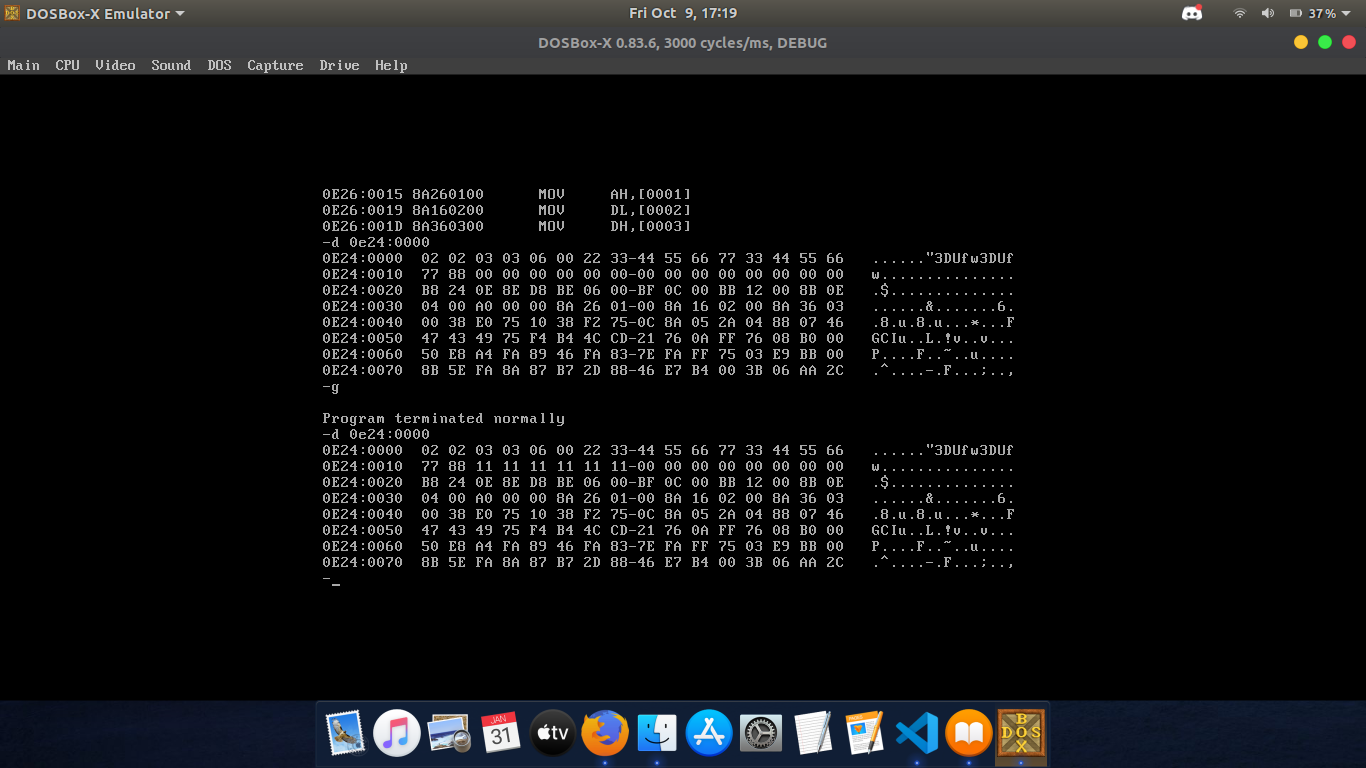
\includegraphics[trim = 100mm 60mm 100mm 80mm, clip, width = \textwidth]{Pics/MSIO.png}
    \caption{ \textbf{Input:} \emph{mat1:} 22H, 33H, 44H, 55H, 66H, 77H; \emph{mat2:} 33H, 44H, 55H, 66H, 77H, 88H ; \newline \hspace{1cm}
              \textbf{Output:} \emph{mat3:} 11H, 11H, 11H, 11H, 11H, 11H}
\end{figure}
\hrule
\subsection*{\textbf{Result:}}
The 8086 programs were written to perform matrix operations, and the results observed.
\end{flushleft}
\end{document}